%==============================================================================
% Template research proposal bachelor thesis
%==============================================================================

\documentclass[english]{hogent-article}

\usepackage{lipsum} % For blind text

% Specify bibliography file
\addbibresource{voorstel.bib}

% Information about the study programme, course, assignment
\studyprogramme{Professional bachelor applied computer science}
\course{Research Methods}
\assignmenttype{Paper Research Methods: research proposal}
\academicyear{2022-2023}

% TODO (phase 1): Working title
\title{Elder Speak Monitor: Increasing accuracy of elderspeech detection using noise reduction and silence detection on audio recordings.}

% TODO (phase 1): Student name and email address
\author{Benjamin Daems}
\email{benjamin.daems@student.hogent.be}

% TODO (phase 1): Co-author name and email address
% If you write the proposal in collaboration with another student, give their
% name and e-mail address here. If you write the proposal alone, remove these
% lines or comment them out.

% TODO (phase 1): Give the link to your Github-repository here
\projectrepo{https://github.com/BenjaminDaems/rm-paper-en}

% Within which specialization from the final year of the study programme
% is this research situated? Choose from this list:
%
% - Mobile \& Enterprise development
% - AI \& Data Engineering
% - Functional \& Business Analysis
% - System \& Network Administrator
% - Mainframe Expert
% - If the research does not fit within one of these domains, specify it
%   yourself
%
\specialisation{Data science \& AI}
\keywords{Speech recognition, speech analysis, Elder Speak}

\begin{document}

\begin{abstract}
This paper is a continuation of a project that aims to reduce unintentional use of derogatory or demeaning speech patterns in caregivers and caregiver trainees working in elder care.
Typical markers of these speech patterns, or Elder Speak (ES) are increased speech volume and pitch, decreased speech tempo, decreased grammatical complexity and repetitive word use.
Volume and pitch have been successfully detected in previous iterations of the project, and detection of the speaker's vocabulary has also been attempted, with a lesser degree of success.
Thus the focus of this paper will be detecting the speech tempo, as well as researching techniques to increase vocabulary detection success rates.
The results of this research will provide a solution to detecting and analyzing speech tempo and give insight in several techniques that may provide better ES detection based on the speaker's vocabulary uses. 
\end{abstract}

\tableofcontents

\bigskip

% TODO: Are you also taking on the Bachelor's thesis this year? Then uncomment
% the text below and adjust it as appropriate.

\paragraph{Remark}

I'm also taking up the bachelor's thesis this year. The content of this research proposal also serves as the subject for my bachelor thesis. My promoter is (Mr./Mrs.) X.\ Surname.


% Describe any differences and/or improvements in this document compared to your research proposal that you submitted for the Bachelor's thesis.

\begin{itemize}
    \item Expanded the methodology section to include a more detailed description following the guidelines of the research methods course.
    \item Slightly expanded the results / conclusion section and seperated them into two distinct sections.
    \item Translateed the entire document to English due to accidental re-registration for the English version of the course.
\end{itemize}

\section{Introduction}%
\label{sec:Introduction}

By 2050, a staggering 21.1 percent of the world's population will be aged 60 or older, which represents a significant increase compared to 9.2 percent in 1990.

Due to this rise, an increasing number of caregivers are coming into contact with elderly care recipients.

Therefore, it is crucial for these caregivers to be able to meet all the needs of these elderly care recipients.

In order to age successfully, it is important to fulfill the social interaction needs of older adults.

Research has shown that social relationships among the elderly contribute to higher life expectancy~\autocite{Rodriguez-Laso2007} and greater life satisfaction~\autocite{Okamoto2008-eh}.

Although we can conclude that the contact between caregivers and the elderly is extremely important, the current interaction between them is often considered inadequate.

Insufficient time is allocated for meaningful conversations between caregivers and care recipients, and communication with older adults is frequently condescending in nature.

This condescending way of speaking, also known as Elder speech (ES), is often experienced as humiliating and disrespectful, resulting in a significant reduction in the quality of these social interactions.

This bachelor's thesis builds upon previous work by Sibian De Gussem and Arne Govaerts, who both pursued the Applied Computer Science program at HOGENT.

They demonstrated, through a prototype application, that pitch and voice volume are two distinct features that can be monitored.

My intention is to expand and enhance this prototype by adding additional functionalities.

These functionalities include detecting pauses and reducing noise in audio files, detecting elderspeak in real-time, and modifying the current interface to reduce the complexity of the application.

\section{Literature Review}%
\label{sec:literature review}

Example of a reference where the author's name is not part of the sentence \autocite{Moore2002}. Be aware that a citation belongs INSIDE the sentence, and in the first sentence that references that source. NEVER use the cite commands outside of a sentence, or at the end of a long paragraph.

\subsection{Elder Speak}
Elder Speak (ES) is a term used to describe a specific way of speaking that often occurs when addressing an older adult. This manner of speaking is characterized by an increase in voice volume and frequency and is often perceived as condescending~\autocite{SteveBalsis2006}.

Elder speak is a comprehensive term that describes a specific way of speaking, which, according to \cite{Campens2021}, is characterized by the following attributes:

\begin{itemize}
    \item Speaking slowly
    \item Exaggerated intonation
    \item Increased pitch
    \item Elevated voice volume
    \item Simplified language, including the use of diminutives and/or inappropriate nicknames or terms of endearment
    \item Reduced grammatical complexity (e.g., predominantly simple sentences)
    \item Use of collective pronouns (e.g., "we" instead of "you")
    \item Frequent use of (affirmative) interjections
    \item Modified nonverbal behavior (e.g., prolonged eye contact, additional gestures, getting too close)
    \item Frequent clarification and repetition
\end{itemize}

\subsection{Noise Reduction}
Noise reduction is a technique that can help improve sound quality by removing irrelevant data and maximizing the relevance of the underlying structure in the data.
\cite{Sainburg_2021} describe two types of noise in audio files: static noise and non-static or dynamic noise.
Static noise refers to constant noise present, such as the sound of a fan.
Dynamic noise, on the other hand, is noise that is not consistently present, such as the sound of a passing car.
Noisereduce \autocite{Sainburg2022} is a Python library that can be used to reduce noise in audio files.

\subsection{Detection of Silences}
\label{subsec:detection-of-silences}

To effectively detect silences, it is necessary to first provide a definition of what constitutes a silence.
In the context of this research project, a silence is defined as a period in which there is no speech present in the recording.
The presence of background noises is not considered as part of the silence.
Additionally, residual sounds that are not loud enough to be registered as speech are not included.

\medskip

To achieve this, it is important to remove as much non-speech content from the recordings as possible.
This can be accomplished by using the noise filter discussed in the previous section.

\medskip

Once the recording is filtered, all remaining audio values in the recording are checked and removed if they fall below a certain threshold value.
This method of aquireing this threshold is yet uncertain, and shall be investigated in the proposed research.

\section{Methodology}%
\label{sec:methodology}


The existing ES application, developed by \cite{DeGussem2022}, has already received positive feedback from the co-promoter, J. Campens, due to its useful functionalities. However, client feedback indicated that the application was too complex to use.

Comparing regular speech and Elder Speak was made difficult by the fact that the analysis took place on two separate pages, requiring copy-paste actions.

To reduce this complexity, the application will be streamlined from 5 pages to a total of 2 pages, namely a page for recording or uploading audio files and a page to display the analysis of these audio files.

Furthermore, practical tests of the existing application revealed that noise and silence were not adequately taken into account during the analysis of audio files.

This negatively influenced the results and will be addressed in the research project.

The silences in the audio files will also be displayed as an additional feature that can assist in determining Elder Speak.

\subsection*{Plan of action}
\label{subsec:plan-of-action}

\textbf{Phase 1: Create noise reduction pipeline}

\textbf{Goal:} Reduce excess noise from audio samples containing both normal speech and potential elder speech.

\textbf{Approach:}
\begin{itemize}
    \item Identify and implement a suitable noise reduction algorithm.
    \item Apply the noise reduction algorithm to audio samples containing normal and potential elder speech.
\end{itemize}

\textbf{Result, deliverable(s):} Both input audio samples now have a reduced amount of noise compared to the original audio samples.

\textbf{Phase 2: Detect useful audio parameters}

\textbf{Goal:} Analyze audio sample volume, audio sample pitch, and the total combined silence duration of each sample.

\textbf{Approach:}
\begin{enumerate}
    \item Extract audio sample volume:
    \begin{itemize}
        \item Apply a volume estimation algorithm to calculate the amplitude or intensity of the audio samples.
        \item Normalize the volume values to a standardized scale for comparison.
    \end{itemize}
    \item Extract audio sample pitch:
    \begin{itemize}
        \item Apply a pitch estimation algorithm to determine the fundamental frequency of the audio samples.
        \item Convert the fundamental frequency to a pitch representation (e.g., note or semitone scale).
    \end{itemize}
    \item Measure the total combined silence duration:
    \begin{itemize}
        \item Detect and analyze periods of silence within the audio samples.
        \item Calculate the duration of each silence period.
        \item Sum up the durations to obtain the total combined silence duration for each audio sample.
    \end{itemize}
\end{enumerate}

\textbf{Result, deliverable(s):} Audio parameters (volume, pitch, silence) of both normal speech and potential elder speech audio samples.

\textbf{Phase 3: Detect elder speech based on audio parameters}

\textbf{Goal:} Compare the audio parameters obtained in Phase 2 to detect potential elder speech.

\textbf{Approach:}
\begin{itemize}
    \item Define thresholds or criteria for each audio parameter that indicate potential elder speech. These thresholds are determined by looking at differences between the normal speech and the elder speech sample.
    \item Compare the extracted audio parameters from Phase 2 against the defined thresholds.
    \item Identify audio samples that meet the criteria for potential elder speech based on the parameter comparisons.
\end{itemize}

\textbf{Result, deliverable(s):} Identification of audio samples that exhibit characteristics suggesting potential elder speech based on the comparison of audio parameters.

\textbf{Visualization}

\begin{figure}[ht]
    \centering
    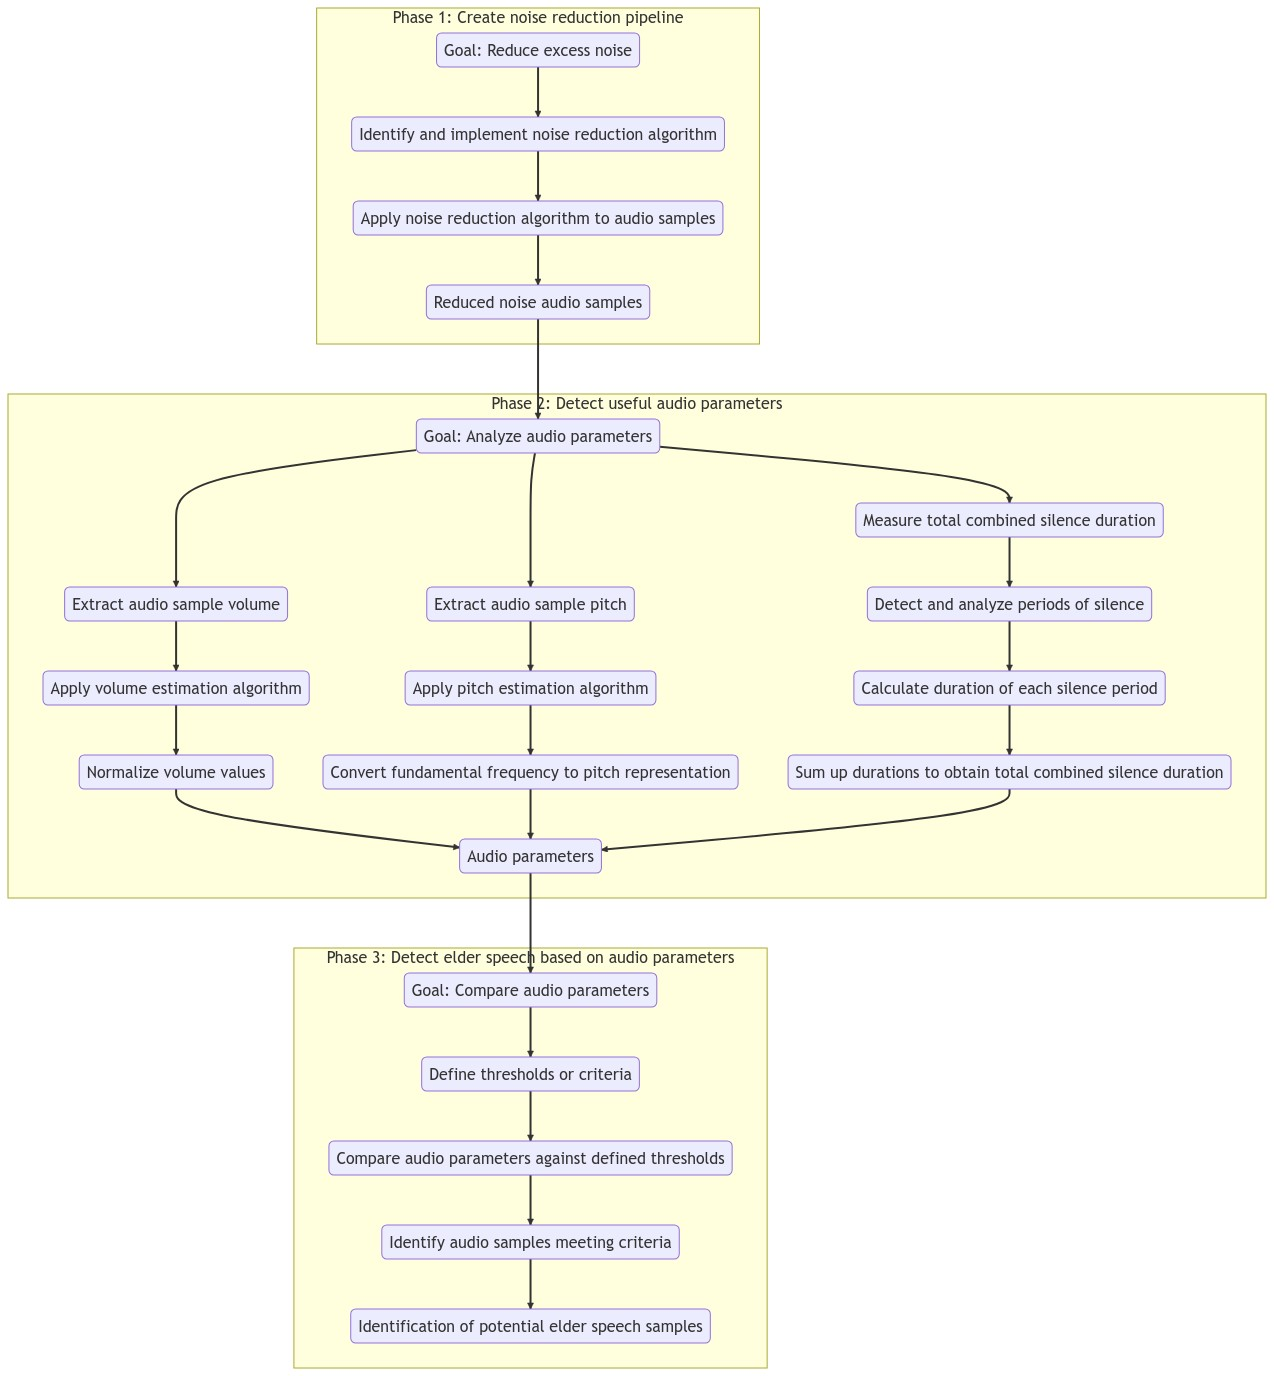
\includegraphics[width=\linewidth]{img/actionplan.png}
    \caption{Visual representation of the process}
\end{figure}


\paragraph{Technologies}
\label{par:technologies}

The current application uses the Python framework Flask and the Python libraries ssl, numpy, librosa, and speech-recognition.

Since the application has already been approved by the client, it will be further developed based on the existing codebase, and therefore, these technologies will be reused.

In addition, the library "noisereduce" \autocite{Sainburg2022} mentioned in the literature review will be used to reduce noise in the audio samples.


\section{Expected results}%
\label{sec:expected-results}

The expected results of the research are the simplification of the ES application from 5 pages to 2 pages and an improvement in the accuracy of the analysis of audio files by considering noise and silence.

Additionally, the application will display the silences in the audio files as an additional feature to facilitate the determination of Elderspeak.

These improvements will simplify the use of the application and enhance the accuracy of the results.

Based on these modifications, it is expected that the ES application will be better able to detect Elderspeak, even in the presence of noise and silence.

The reduction in the number of pages will significantly decrease the complexity of the application, making it easier for users to perform the analysis of audio files.

In summary, these enhancements will contribute to the user-friendliness and accuracy of the ES application.

\section{Discussion, conclusion}%
\label{sec:discussion-conclusion}

In conclusion, the expected results of this research suggest that the simplification of the application, along with the reduction of noise and inclusion of silence detection, will significantly enhance the quality of elder speech detection. These improvements will improve the usability and accuracy of the ES application, benefiting researchers and professionals engaged in the study of elder speech analysis.

%------------------------------------------------------------------------------
% Bibliography
%------------------------------------------------------------------------------
% TODO: (phase 4) the referenced works must be in a BibTeX file references.bib.
% Use JabRef to edit the bibliography file.

\printbibliography[heading=bibintoc]

\end{document}